%
\section{Use of the database}
\label{database_usage}

This section provides an overview of the database interface and of the different
tables available for each simulation. Simple examples of how to query and
combine the tables are presented.

\subsection{Database interface}

The main interface to the \eagle database is shown in
Figure~\ref{fig:interface_example}. Users familiar with the {\it Millennium}
database \citep{Lemson2006b} and its clones will recognize the main features of
the interface and should be able to adapt their scripts easily to the \eagle database.

\sql queries can be typed in the main text box (number 1 in the Figure) and are
submitted to the database by pressing either of the buttons to the right (number
2). Some help with \sql queries can be obtained by clicking on the corresponding
button. The results of queries submitted to the \emph{browser} are returned at
the bottom of the page in the form of an HTML table\footnote{Note that the
  \emph{browser} queries time out after $90$ seconds. More substantial queries
  should be submitted via the \emph{stream} queries option. These only time out
  after $30$ minutes.} (number 7). This allows users to submit small queries and quickly
verify the syntax. If images are being queried, they will appear directly in the
results table. Larger, more complex queries should be submitted to the
\emph{stream} and will be returned in Comma-Separated-Value (CSV) format in a
new window. The number of rows returned by the \emph{browser} queries can be
specified via the drop-down menu (number 3). The \emph{stream} queries always
return all rows. Previous queries can be recovered using the drop-down
menu (number 4).

The queries from this paper are available as examples (number 5). These can
later be adapted to match the user's need. All the available simulations and
their tables are listed in the left-hand panel (number 6) with links to the
documentation describing each entry in the table. All registered users receive a
private database (MyDB) in which they can store query results for further
processing at a later date. A link to MyDB is provided (number 11). Examples of
how to create and manage such private tables can be obtained by clicking on the
buttons at the bottom of the screen (number 8). Finally, some documentation, a
list of credits are given at the top of the page (numbers 9 \& 10).


\begin{figure*}  [p]
\centering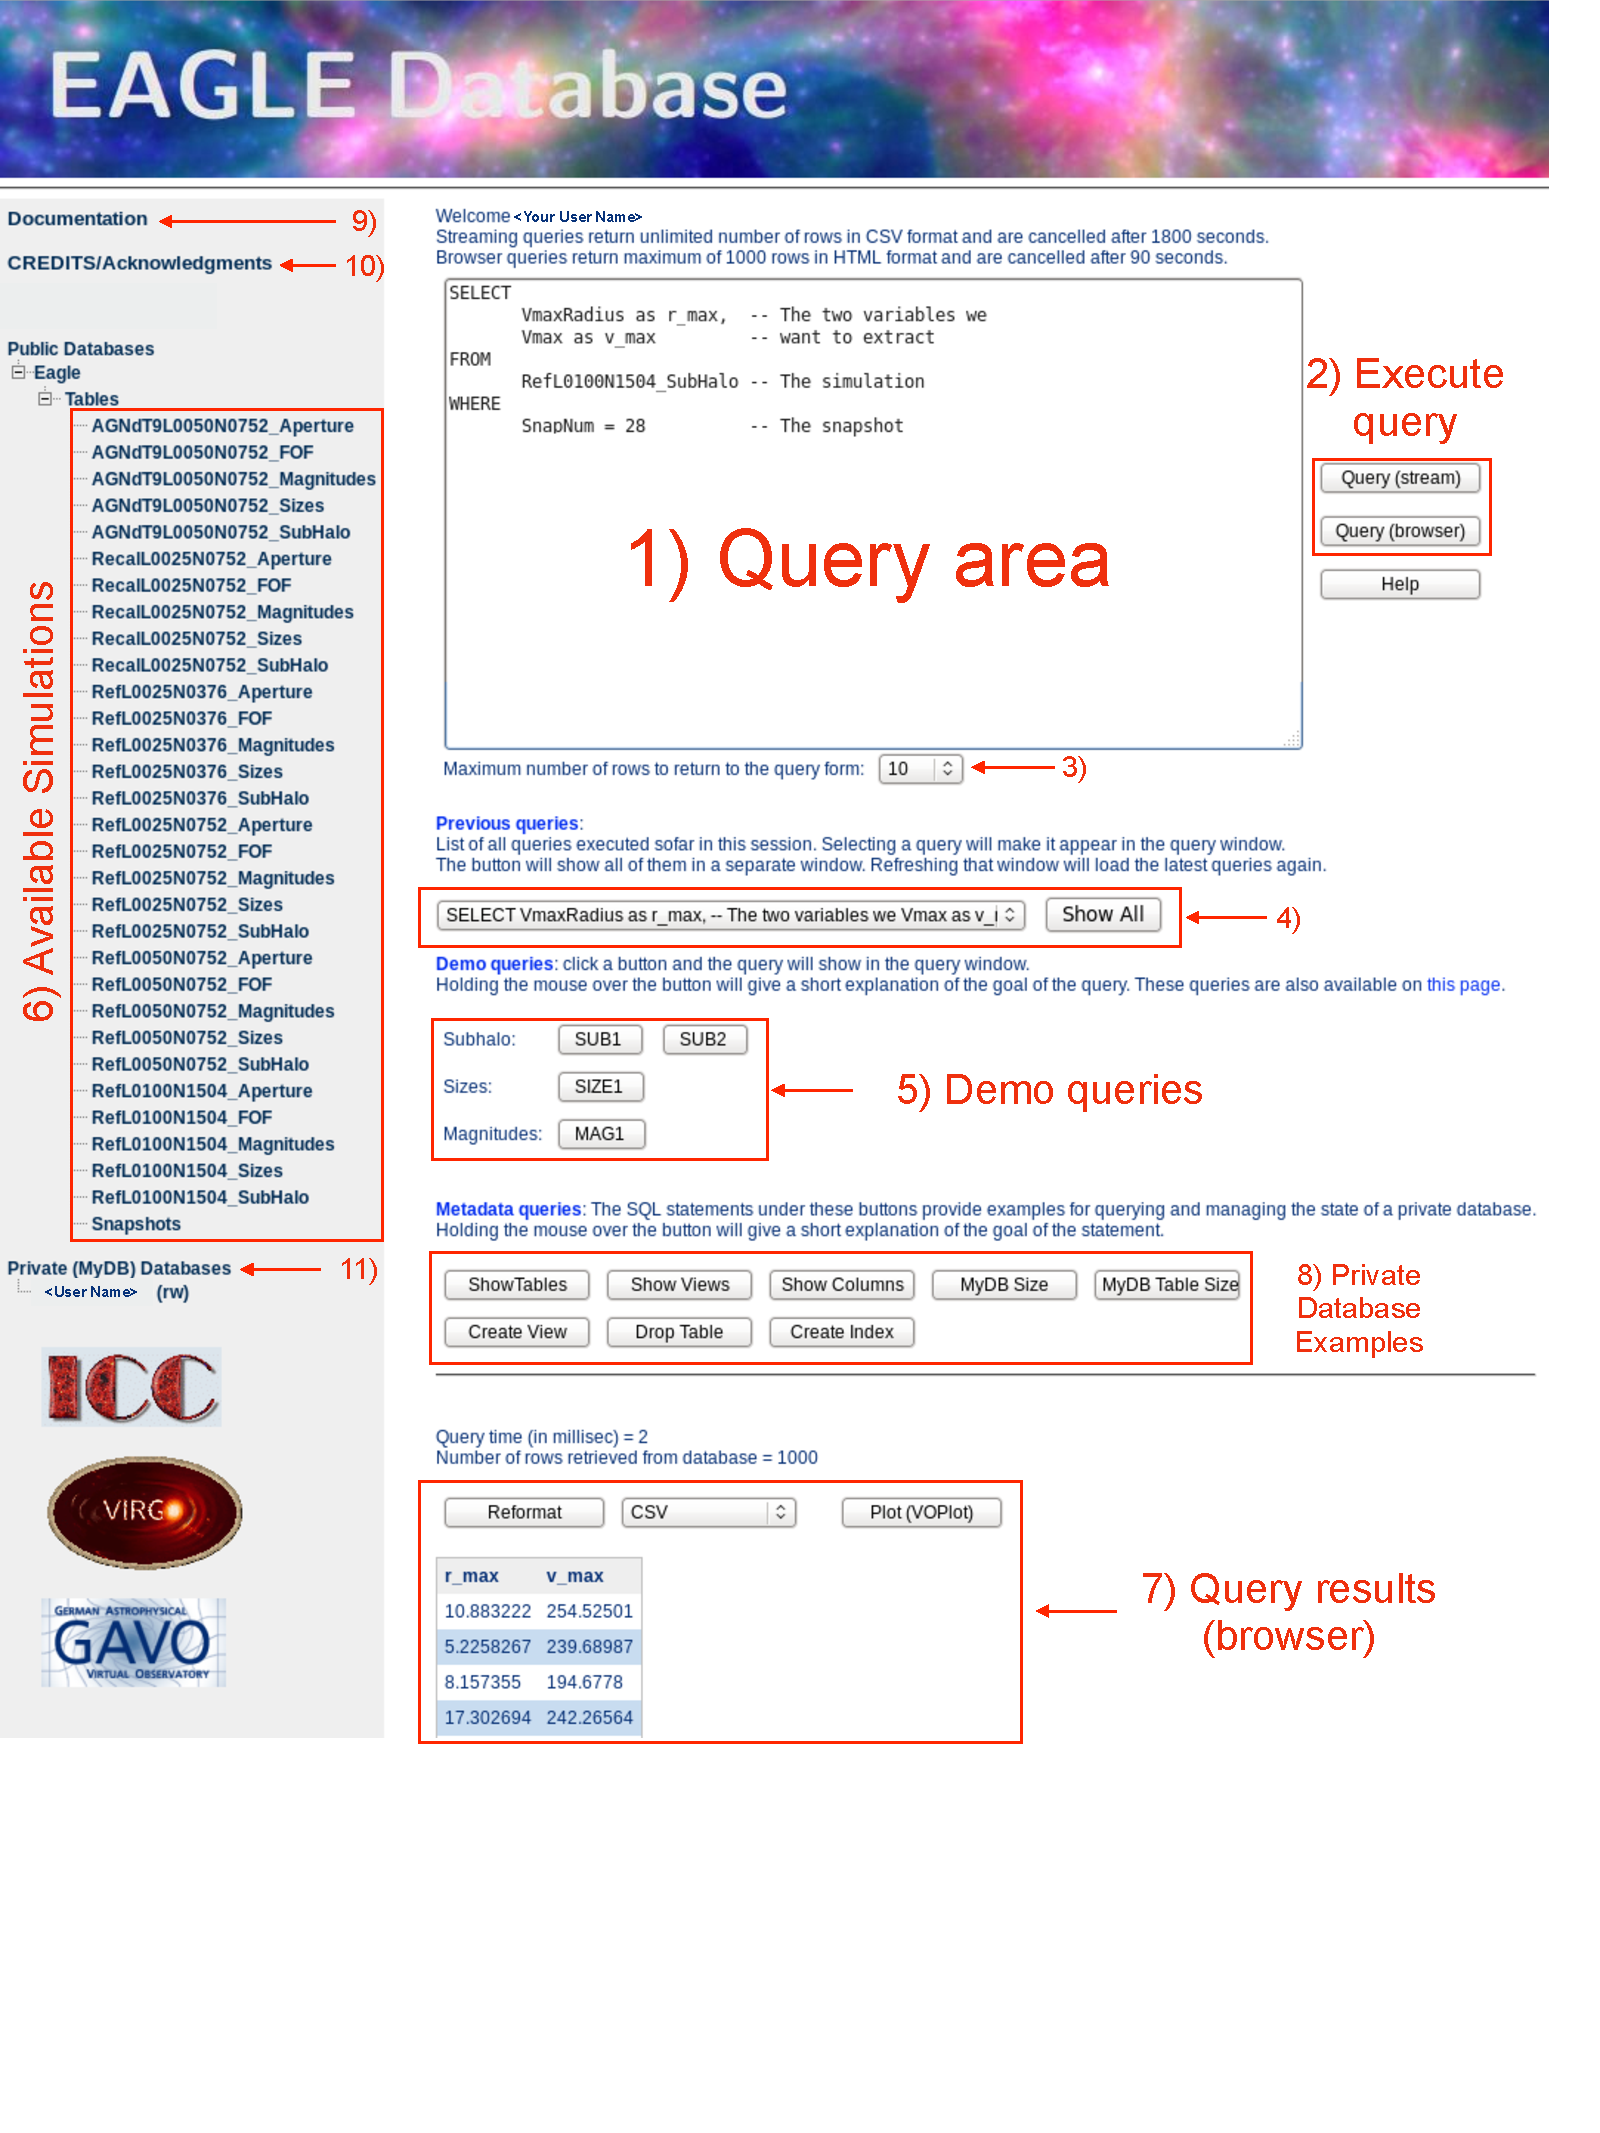
\includegraphics[width=0.98\textwidth]{figures/interface_example.pdf}
\caption{The interface of the \eagle database. \sql queries should be entered
  into the query area (1) and can be executed either via the \squotes{browser}
  or \squotes{stream} buttons (2). The \emph{browser query} returns a limited
  number of results (3) at the bottom of the page (7), pressing the
  \emph{Reformat} button will then return the full results in the selected
  format (default CSV) and \emph{Plot(VOPlot)} is a simple way to visualise the
  data. This is the easiest method to test \sql scripts. The \emph{stream query}
  returns all the results in a CSV format in a separate window to ease their
  download to a local device. Previous queries can be restored from the
  drop-down menu (4). The example query buttons (5) insert example \sql
  queries into the query area to help new users with the syntax and structure of
  the database. Similarly, examples creating and managing a private database are
  generated by clicking on the buttons (8). The list of available simulations
  and tables is given on the left hand side (6) with links to further
  documentation describing their contents.  Users' own database tables are
  listed below (11). Further step-by-step documentation on how to use the web
  interface is provided (9) as well as links pointing to credits and
  acknowledgements (10). }
\label{fig:interface_example}
\end{figure*}


\subsection{Galaxy merger-tree traversal}
In order to simplify the navigation of the trees, the database is stored with
depth-first ordering \citep[see][Qu et al., \textit{in prep.}]{Lemson2006a}. The
progenitors of a galaxy can then easily be identified. To allow simple
traversing of the merger tree of a given galaxy (with its unique \HaloID), three
additional columns are assigned to each galaxy:
\begin{enumerate}
\item \TopLeafID: This is the \HaloID of the highest-redshift main branch
  progenitor. \\ 
  All the galaxies on the \emph{main progenitor branch} of a galaxy with \HaloID $i$
  and \TopLeafID $j$ have a \HaloID in the range $[i,j]$ in ascending redshift order.
\item \LastProgID: This is the maximum \HaloID of all progenitors irrespective
  of their branch. \\
  All the galaxies on \emph{any progenitor branch} of a galaxy with \HaloID $i$
  and \LastProgID $k$ have a \HaloID in the range $[i,k]$. 
\item \DescendantID: This is the \HaloID of the unique descendant galaxy of
  $i$. \\
  If no descendant galaxy is identified then the \\ \DescendantID of a galaxy is
  set to its own \HaloID.
\end{enumerate}
In Fig. \ref{fig:mergerTree} we show a merger tree for a typical galaxy,
indicated by its \HaloID. The main branch is shown using a thicker blue line
and the IDs required to navigate the tree are shown with arrows pointing
towards the galaxy to which they correspond in the tree\footnote{Users
  familiar with the \emph{Millennium} database can modify they queries
  by replacing {\tt HaloID} with \GalaxyID, {\tt mainLeafID} or {\tt
    endMainBranchID} with \TopLeafID and {\tt lastProgenitorId}
  with \LastProgID. Note also that in the \emph{Millennium} database, a
galaxy with no descendant has its \DescendantID set to -1 and not to
\GalaxyID as in the \eagle database.} . \\ Examples using the
\sql language showing how to traverse the tree forwards and backwards in time
are provided in \ref{example_scripts}.







\subsection{Content of the database}
The \eagle database for each simulation has information distributed
across five \sql \lq tables\rq\ listed in Table~\ref{table_tables}, whose
contents are detailed in \ref{appendix_quantities}. \\


\begin{table}
\footnotesize
\begin{center}
\renewcommand{\arraystretch}{1.5}
\begin{tabular}{ll}
\hline
\sql Table name & Contents \\
\hline\hline
{\bf SubHalo} & Main galaxy properties \\
{\bf FOF} & Halo properties\\
{\bf Sizes} & Galaxy sizes \\
{\bf Aperture} & Galaxy properties in 3D apertures \\
{\bf Magnitudes} & Galaxy photometry in the GAMA bands\\
\hline
\end{tabular}
\end{center}
\caption{\sql tables available for each simulation. The tables are prefixed with
  the name of the simulation to which they correspond. For example, the table of
  magnitudes for the 50~Mpc Ref- model is labelled {\bf
    RefL0050N0752\_Magnitudes} as can be seen on Figure
  \ref{fig:interface_example}.}
\label{table_tables}
\end{table}


{\bf SubHalo:} This is the main table containing properties of {\em galaxies},
for example masses (of dark matter, gas, stars, and black holes), star formation
rates, metallicities and angular momentum. The \GalaxyID of a galaxy can be used
to navigate through its descendants and progenitors as well as to join the
galaxy property table to other tables containing additional properties. The
examples below demonstrate how to do this.\\ A full description of the contents
of the {\bf SubHalo} table is given in Table \ref{table:subhalo1}.\\

{\bf Aperture:} This table contains masses, star formation rates and velocity
dispersions measured in a range of spherical apertures. Table \ref{table:aperture}
gives a full list of the fields present in that \sql table. This table can be
joined to the {\bf SubHalo} table via the \GalaxyID of the objects. \\

{\bf Magnitudes:} This table contains non-dust-attenuated rest-frame broad-band
magnitudes in the SDSS $ugriz$ filters \citep{SDSSfilters} and in the UKIRT
$YJHK$ filters \citep{UKIRTfilters}, computed in 30~pkpc spherical apertures for
all galaxies with stellar mass greater than $10^{8.5}\Msol$ as described in
\cite{Trayford2015}.  See Table \ref{table:magnitudes} in the appendix for more
details. This table can be joined to the {\bf SubHalo} table via the \GalaxyID
of the objects. \\

{\bf Sizes:} This table contains half-mass sizes of galaxies computed starting
from apertures, as presented in Furlong et al., ({\it in prep.}). See Table
\ref{table:sizes} in the appendix for a full list of available quantities. This
table can be joined to the {\bf SubHalo} table via the \GalaxyID of the
objects. \\

{\bf FOF:} This table contains properties of {\em haloes}, for example mass and
spherical overdensity radii. A full description of the contents of the FOF group
table, including the units and dimensions of each variable, is given in Table
\ref{table:fof}. This table can be joined to the {\bf SubHalo} table via the
    {\tt GroupID} of the galaxies, given in the {\bf SubHalo} table. \\


The {\bf FOF} and {\bf SubHalo} tables also contain a field with random number
uniformly distributed in the range $[0,1)$ allowing the users to generate
  unbiased sub-samples of galaxies or haloes.


\subsection{Querying the database tables}
In this section we will illustrate the use of the database by
presenting simple example queries showing the basic usage of the different
\sql tables. \\

The queries can be typed directly into the web interface or used in a {\sc
  Python} script, as described in \ref{example_scripts}, or using the UNIX {\tt
  wget} command as described in the online documentation. The first example
illustrates how to query the main galaxy table ({\bf SubHalo}) in order to plot
the relation between $r_{\max}$ and $v_{\rm max}$ at $z=0$ ({\tt Snapnum}$~=28$)
for the Ref-L0100N1504 simulation. In the database nomenclature, these
quantities are {\tt VmaxRadius} and {\tt Vmax} (see Table \ref{table:subhalo2}).

\noindent 
The \sql command to be typed in the input window is
{
\sqlstyle
{
\footnotesize
\begin{lstlisting}[numbers = none,caption={Generate
      $r_{\max}$-$v_{\max}$ table at $z=0$}]
SELECT        
   VmaxRadius as r_max,  -- The two variables we
   Vmax as v_max         -- want to extract
FROM 
   RefL0100N1504_SubHalo -- The simulation
WHERE  
   SnapNum = 28          -- The snapshot 
\end{lstlisting}
}
}
\noindent Clicking on the ``Query (stream)'' will open a new window containing
the resulting two-column table with headers ``r\_max'' and ``v\_max''
in CSV format. \\


For many applications, multiple \sql tables have to be queried at the same
time. The properties of a galaxy can be retrieved across the tables by joining
their \GalaxyID. A rest-frame colour-magnitude diagram using the SDSS $g$ and
$r$ bands at $z=0.1$ ({\tt SnapNum}~$=27$) for central galaxies ({\tt
  SubGroupNumber}$~=0$) with a stellar mass larger than $10^9\Msol$ ({\tt
  Mass\_Star}~$>{\mathtt{1.0e9}}$) in a $30~\rm{pkpc}$ aperture ({\tt
  ApertureSize}~$=30$) can be constructed by joining the {\bf SubHalo} table to
the {\bf Magnitudes} and {\bf Aperture} ones.

This query reads
{
\sqlstyle
{
\footnotesize
\begin{lstlisting}[numbers = none,caption={Generate
      table of $g-r$ vs. $r$ colour-magnitude table for central
      galaxies with $M_*>10^9$ at $z=0.1$}]
-- Select the quantities we want
SELECT        
   (MAG.g_nodust - MAG.r_nodust) as g_minus_r,
   MAG.r_nodust as r
-- Define aliases for the three tables
FROM 
   RefL0100N1504_SubHalo as SH,
   RefL0100N1504_Magnitudes as MAG,
   RefL0100N1504_Aperture as AP
-- Apply the conditions
WHERE  
   SH.SnapNum = 27 and        -- z=0.1
   SH.SubGroupNumber = 0 and  -- Centrals only
   AP.Mass_Star > 1.0e9 and  -- Mass limit
   AP.ApertureSize = 30 and  -- Aperture size
-- Join the objects in the 3 tables
   SH.GalaxyID = MAG.GalaxyID and
   SH.GalaxyID = AP.GalaxyID
\end{lstlisting}
}
}
\noindent and will return a two-column table with ``g\_minus\_r'' and ``r'' as
headers containing the colours and $r$-band magnitudes of the selected
galaxies.

Note that, as discussed in Section~\ref{caveats}, we recommend to always use
quantities measured in apertures to avoid incorporating intra-cluster light into
mass or star formation rate estimates. \\

Another common use of the database is to track one galaxy across time. To this
end, one can navigate through the main progenitor branch. This final example
tracks an interesting object (\GalaxyID$=1848116$) discovered at redshift $z=1$
through time and constructs the stellar metallicity evolution accompanied by
the mock $gri$ face-on images of the object at all redshifts. One hence has to
construct a query that returns all of the descendants (on the main branch) of
the object by finding all galaxies that have the interesting object's \GalaxyID
between their own \GalaxyID and their {\tt TopLeafID}. To get the progenitors
one additionally requests all galaxies with \GalaxyID between the interesting
object's \GalaxyID and its {\tt TopLeafID}.  This demonstrates the merger tree
navigation introduced in Section \ref{subsection:merger_trees}. Note that
adding conditions on the snapshot number ({\tt SnapNum}) helps speed up the
queries dramatically. This query reads

{
\sqlstyle
{
\footnotesize
\begin{lstlisting}[numbers = none,caption={Returns the evolution along the main
branch of stellar metallicity with redshift of a given galaxy with its images.
To return the evolution along all branches replace \tt{TopLeafID} with
\tt{LastProjID} in line 20.}]
-- Select the quantities we want
SELECT      
   SH.Redshift as z,      
   SH.Stars_Metallicity as Z,      
   SH.Image_Face as face      
-- Define two aliases for the main table
FROM      
   -- Properties we want to extract      
   RefL0025N0752_Subhalo as SH,      
   -- Acts as a reference point      
   RefL0025N0752_Subhalo as REF      
-- Apply the conditions      
WHERE      
   REF.GalaxyID=1848116 and -- GalaxyID at z=1      
   -- To find descendants      
   ((SH.SnapNum > REF.SnapNum and REF.GalaxyID      
   between SH.GalaxyID and SH.TopLeafID) or 
   -- To find progenitors  
   (SH.SnapNum <= REF.SnapNum and SH.GalaxyID  
   between REF.GalaxyID and REF.TopLeafID))  
-- Order the output by redshift      
ORDER BY      
   SH.Redshift
\end{lstlisting}
}
}
\noindent and will return a sorted table with a redshift and a metallicity
column as well as a column containing the postage-stamp images of the galaxy at
each redshift when using the ``Query (browser)'' button. These examples along with
the more complex queries are given in \ref{example_scripts} are listed on the
webpage documentation.
